% Provenance (never printed): see sources/outline_sources.md (Year 3:
% geophysical fluid dynamics: rotating-frame equations, Rossby number,
% hydrostatic and geostrophic balance, thermal wind, buoyancy frequency).
% Brief: sources/book5/BRIEFS.md, ch. 19. Curves from
% figdata/bachelor-3/inertial_oscillation.py, thermal_wind.py and
% buoyancy_frequency.py. Exercise and problem values in the Book 5 scratch
% calculator calc/ch19.py. The Steppe of Orrin, its lake, its stations and
% its winds are invented.
\chapter{Dinâmica de fluidos geofísicos}\label{ch:b3:gfd-foundations}

Mexa uma xícara de chá e o redemoinho se desfaz em um minuto; as folhas se juntam no
centro do fundo e nada mais acontece. O oceano e a atmosfera
também são agitados, pelo Sol e pelo vento, mas em um planeta em rotação e em
camadas de densidades diferentes. Rotação e estratificação os fazem obedecer a
regras que uma xícara de chá nunca mostra: os ventos sopram ao longo das isóbaras em vez de
atravessá-las, colunas de fluido se recusam a inclinar-se, e o vento da alta
troposfera está inscrito nas temperaturas abaixo dele. Este capítulo estabelece
as equações desses escoamentos grandes, lentos e rasos e os poucos números que
decidem quais termos importam.

\begin{recall}
As forças de Coriolis e centrífuga em um referencial girante, as equações de Navier--Stokes
e da continuidade, a viscosidade, o número de Reynolds e a relação hidrostática
estão nos livros de física. O parâmetro de Coriolis $f = 2\Omega
\sin\varphi$, a força do gradiente de pressão, o equilíbrio geostrófico, os
ventos geostróficos e gradiente e as correntes de jato estão no volume do primeiro
ano, no seu capítulo sobre a circulação geral da atmosfera; a
camada de Ekman no seu capítulo sobre a circulação do oceano; a temperatura potencial,
a estabilidade estática e a oscilação de uma parcela de ar elevada, no seu
capítulo sobre a estrutura da atmosfera e do oceano.
\end{recall}

\section{Equações em um referencial girante}\label{sec:b3:gfd-foundations:equations}

Em um referencial que gira com a Terra, à velocidade angular
$\vec\Omega$, uma parcela de fluido de velocidade $\vec u$ obedece a
\[
\frac{\mathrm D\vec u}{\mathrm Dt} + 2\vec\Omega\times\vec u =
-\frac{1}{\rho}\nabla p + \vec g + \nu\nabla^2\vec u ,
\qquad
\frac{\partial\rho}{\partial t} + \nabla\cdot(\rho\vec u) = 0 ,
\]
onde $\mathrm D/\mathrm Dt = \partial/\partial t + \vec u\cdot\nabla$ é
a derivada seguindo a parcela e $\nu$ a viscosidade cinemática. A força
centrífuga foi somada à gravitação: a soma delas, $\vec g$, é a
gravidade efetiva, normal às superfícies de nível do \omterm{def:b3:gravity-geodesy:geopotential}{geopotencial}, e
a vertical é definida por ela. Da rotação resta apenas o termo de Coriolis, $-2\vec\Omega\times
\vec u$, que não realiza trabalho: ele desvia uma parcela
sem alterar sua velocidade. A Terra gira a $\Omega =
\qty{7.292115e-5}{rad/s}$, uma vez por dia sideral de \qty{23.9345}{h}.
% ledger: geod5:grs80-defining, earth:Trot

Para movimentos em distâncias muito menores que o raio da Terra $a$, um
referencial cartesiano local é suficiente: $x$ para leste, $y$ para norte, $z$ para
cima, na latitude $\varphi$, o plano tangente da figura abaixo. Ali
$\vec\Omega = \Omega\,(0, \cos\varphi, \sin\varphi)$, e as três
componentes da equação do momento são
\[
\begin{aligned}
\frac{\mathrm Du}{\mathrm Dt} - f v + \tilde f w &= -\frac{1}{\rho}\frac{\partial p}{\partial x} + F_x ,\\
\frac{\mathrm Dv}{\mathrm Dt} + f u &= -\frac{1}{\rho}\frac{\partial p}{\partial y} + F_y ,\\
\frac{\mathrm Dw}{\mathrm Dt} - \tilde f u &= -\frac{1}{\rho}\frac{\partial p}{\partial z} - g + F_z ,
\end{aligned}
\qquad f = 2\Omega\sin\varphi,\quad \tilde f = 2\Omega\cos\varphi ,
\]
com $\vec F$ o atrito. Para os escoamentos finos e quase horizontais do
oceano e da atmosfera, os termos em $\tilde f$ são desprezados: $\tilde f w$
é pequeno diante de $fv$ porque $w \ll v$, e $\tilde f u$ é a dez-milésima parte
de $g$ (veja o \cref{exo:b3:gfd-foundations:5}). A força de Coriolis então atua apenas
na horizontal, por meio da componente vertical local da rotação,
$\Omega\sin\varphi$.

\begin{definition}[plano $f$ e plano $\beta$]\label{def:b3:gfd-foundations:planes}
Próximo de uma latitude de referência $\varphi_0$, a aproximação do \emph{plano $f$}\index{f-plano@plano $f$}
toma o parâmetro de Coriolis como constante, $f = f_0 =
2\Omega\sin\varphi_0$. A aproximação do \emph{plano $\beta$}\index{beta-plano@plano $\beta$}
mantém sua variação de primeira ordem com a distância para o norte $y$:
$f = f_0 + \beta y$, com $\beta = \mathrm df/\mathrm dy = 2\Omega
\cos\varphi_0/a$.
\end{definition}

Em \ang{45}, com o raio médio $a = \qty{6371}{km}$, $f_0 =
\qty{1.031e-4}{s^{-1}}$ e $\beta = \qty{1.62e-11}{m^{-1}.s^{-1}}$: em
\qty{1000}{km} de latitude $f$ muda \qty{16}{\percent}. O plano $f$
serve a movimentos bem menores que isso; o plano $\beta$ é necessário para
correntes de escala de bacia e ondas planetárias.
% ledger: earth:Rmean, geod5:grs80-defining (values in figdata/bachelor-3/inertial_oscillation.py)

\begin{omfigure}
\begin{minipage}[c]{0.42\linewidth}\centering
\begin{tikzpicture}[>=stealth, font=\small]
\draw[thick] (0,0) circle (2);
\draw[black!40, dashed] (-2,0) -- (2,0);
\draw[->, thick] (0,-2.4) -- (0,2.75) node[above] {$\vec\Omega$};
\draw (0,0) -- (30:2) coordinate (P);
\draw (0.6,0) arc (0:30:0.6);
\node at (15:0.9) {$\varphi$};
\draw[black!60] ($(P)+(120:-1.1)$) -- ($(P)+(120:1.3)$);
\draw[->, omThm, thick] (P) -- ++(0,1.6) node[right] {$\vec\Omega$};
\draw[->, omDef, thick] (P) -- ++(30:0.8) node[anchor=south west, align=left, inner sep=1pt] {$\Omega\sin\varphi$,\\ para cima};
\draw[->, omMeth, thick] (P) -- ++(120:1.386) node[anchor=south, align=center, inner sep=1pt] {$\Omega\cos\varphi$,\\ para norte};
\draw[black!50, densely dotted] ($(P)+(30:0.8)$) -- ($(P)+(0,1.6)$) -- ($(P)+(120:1.386)$);
\draw (P) circle (0.09); \draw ($(P)+(-0.064,-0.064)$) -- ($(P)+(0.064,0.064)$);
\draw ($(P)+(-0.064,0.064)$) -- ($(P)+(0.064,-0.064)$);
\node[font=\scriptsize, anchor=west] at ($(P)+(0.14,-0.03)$) {$x$, leste};
\node[font=\scriptsize, black!60] at (-1.15,-0.25) {equador};
\end{tikzpicture}
\end{minipage}\hfill
\begin{minipage}[c]{0.55\linewidth}\centering
\begin{tikzpicture}
\begin{axis}[width=\linewidth, height=0.72\linewidth, xmin=0, xmax=90, ymin=0, ymax=1.8,
  xlabel={latitude (\unit{\degree})}, ylabel={$f$ ($10^{-4}$\,\unit{s^{-1}})},
  xtick={0,15,30,45,60,75,90}, tick label style={font=\scriptsize}, label style={font=\small},
  legend style={font=\scriptsize, draw=none, fill=none}, legend pos=north west]
% computed in figdata/bachelor-3/inertial_oscillation.py
\addplot[omDef, thick] table[x=lat, y=f] {figdata/out/bachelor-3-inertial_oscillation-fbeta.dat};
\addplot[omThm, densely dashed] table[x=lat, y=fb] {figdata/out/bachelor-3-inertial_oscillation-fbeta.dat};
\addplot[only marks, mark=*, mark size=1.6pt] coordinates {(45,1.03126)};
\legend{$2\Omega\sin\varphi$, plano $\beta$ a \ang{45}}
\end{axis}
\end{tikzpicture}
\end{minipage}

\par\smallskip{\small À esquerda, o referencial local na latitude $\varphi$: $z$
ao longo da vertical local, $y$ para o norte no plano tangente, $x$ para leste
entrando na página. O vetor de rotação se decompõe em $\Omega\sin\varphi$ em torno da
vertical, que faz girar o movimento horizontal, e $\Omega\cos\varphi$ em torno do
eixo voltado para o norte, desprezado para escoamentos delgados. À direita, o parâmetro de Coriolis e
seu plano tangente $\beta$ em \ang{45}: próximos numa faixa de latitudes, distantes
dela perto do equador e do polo.}\label{fig:b3:gfd-foundations:frame}
\end{omfigure}
% ledger: geod5:grs80-defining, earth:Rmean

Duas outras aproximações simplificam as equações sem perder o que
importa. A primeira diz respeito à densidade.

\begin{definition}[Aproximação de Boussinesq]\label{def:b3:gfd-foundations:boussinesq}
A \emph{aproximação de Boussinesq}\index{aproximação de Boussinesq} escreve
a densidade como $\rho = \rho_0 + \rho'$, com $\rho_0$ constante e
$|\rho'| \ll \rho_0$, e mantém $\rho'$ apenas onde ela multiplica $g$.
A equação da continuidade torna-se $\nabla\cdot\vec u = 0$, e a equação
do momento
\[
\frac{\mathrm D\vec u}{\mathrm Dt} + f\,\vec k\times\vec u =
-\frac{1}{\rho_0}\nabla p' + b\,\vec k + \nu\nabla^2\vec u ,
\qquad b = -g\,\frac{\rho'}{\rho_0} ,
\]
em que $p'$ é o desvio da pressão em relação à pressão hidrostática
da densidade $\rho_0$, $\vec k$ o vetor unitário para cima e $b$ a
flutuabilidade.
\end{definition}

Na água do oceano, $\rho'$ é de alguns \unit{kg/m^3} sobre \num{1025}, uma fração de
por cento, e a aproximação é excelente. Na atmosfera, a densidade cai por um
fator $e$ em cerca de \qty{8.5}{km}; a aproximação vale para camadas muito
mais finas do que isso, e escoamentos mais profundos substituem $\rho_0$ por um
perfil médio $\rho_0(z)$, com a mesma física.
% ledger: earth:Hscale

A segunda diz respeito à vertical. Um fluido em repouso está em equilíbrio
hidrostático; um fluido em movimento o mantém com muito boa aproximação quando
o movimento é muito mais largo do que profundo.

\begin{definition}[Aproximação hidrostática]\label{def:b3:gfd-foundations:hydrostatic}
A \emph{aproximação hidrostática}\index{aproximação hidrostática}
substitui a equação do momento vertical de um fluido em movimento pela
relação hidrostática, $\partial p/\partial z = -\rho g$.
\end{definition}

\begin{proposition}[Quando a aproximação hidrostática vale]\label{prop:b3:gfd-foundations:hydrostatic}
Para um movimento de escala horizontal $L$, profundidade $H$ e velocidade $U$, com um
\omterm{def:b3:gfd-foundations:numbers}{número de Rossby} $U/(fL)$ no máximo da ordem de um, a aceleração vertical é
menor do que o gradiente vertical da perturbação de pressão por um fator
da ordem de $(U/fL)\,(H/L)^2$.
\end{proposition}

\begin{proof}
Quando a força de Coriolis é pelo menos tão grande quanto a aceleração, a
equação do momento horizontal equilibra o gradiente horizontal de pressão
contra ela: $p'/(\rho_0 L) \sim fU$, logo $p'/\rho_0 \sim fUL$, e o gradiente
vertical é $p'/(\rho_0 H) \sim fUL/H$. A continuidade, $\partial w/\partial z
= -(\partial u/\partial x + \partial v/\partial y)$, limita a velocidade
vertical por $W \sim UH/L$, e a aceleração vertical por
$\mathrm Dw/\mathrm Dt \sim UW/L = U^2H/L^2$. A razão é $(U^2H/L^2)/(fUL/H)
= (U/fL)(H/L)^2$.
\end{proof}

Um sistema meteorológico de \qty{1000}{km} de largura em uma troposfera de \qty{10}{km}
de profundidade tem $(H/L)^2 = 10^{-4}$ e um \omterm{def:b3:gfd-foundations:numbers}{número de Rossby} de cerca de 0.1: o
erro da \omterm{def:b3:gfd-foundations:hydrostatic}{aproximação hidrostática} é da ordem de $10^{-5}$. Ela falha apenas em movimentos
estreitos e profundos: uma corrente ascendente de tempestade, uma pluma convectiva no oceano.

\section{Escalas do escoamento em rotação}\label{sec:b3:gfd-foundations:scales}

Quais termos da equação do momento importam é decidido por duas razões.

\begin{definition}[Números de Rossby e de Ekman]\label{def:b3:gfd-foundations:numbers}
Para um escoamento de velocidade $U$, escala horizontal $L$ e profundidade $H$ em um planeta de
parâmetro de Coriolis $f$, o \emph{número de Rossby}\index{número de Rossby} é
$\mathrm{Ro} = U/(fL)$, a razão entre a aceleração, da ordem de $U^2/L$,
e a força de Coriolis, da ordem de $fU$. O \emph{número de
Ekman}\index{número de Ekman} é $\mathrm{Ek} = \nu/(fH^2)$, a razão entre
a força viscosa, da ordem de $\nu U/H^2$, e a força de Coriolis; em um
escoamento turbulento $\nu$ é substituída por uma viscosidade de turbilhão.
\end{definition}

Um ralo de banheira que escoa \qty{0.1}{m/s} sobre \qty{0.3}{m} tem \omterm{def:b3:gfd-foundations:numbers}{número de Rossby} de
alguns milhares: a rotação da Terra não decide o sentido do seu redemoinho. Uma depressão de
\qty{1000}{km} de diâmetro com ventos de \qty{15}{m/s} tem
$\mathrm{Ro} \approx 0.14$, e um giro oceânico tem $\mathrm{Ro} \sim 10^{-4}$.
A viscosidade é ainda mais fraca: a viscosidade molecular da água é
\qty{e-6}{m^2/s}, e as viscosidades de turbilhão que representam a turbulência
do oceano, \qtyrange{e-5}{e-3}{m^2/s} na vertical, dão
$\mathrm{Ek} \sim 10^{-5}$ ao longo de \qty{1000}{m} de profundidade. Os dois números se
relacionam ao número de Reynolds por $\mathrm{Re} = UL/\nu =
(\mathrm{Ro}/\mathrm{Ek})(L/H)^2$.
% ledger: stewart:eddy (problem values in calc/ch19.py)

Quando os dois números são pequenos, a equação do momento horizontal estacionária mantém
apenas a força de Coriolis e o gradiente de pressão: o escoamento está em
equilíbrio geostrófico, $f\,\vec k\times\vec u_g = -(1/\rho)\nabla_h p$, que o
volume do primeiro ano leu a partir de mapas meteorológicos. A geostrofia é o limite
$\mathrm{Ro}, \mathrm{Ek}\to 0$; suas correções são da ordem de
$\mathrm{Ro}$, e o atrito atua apenas em camadas finas de espessura relativa
$\sqrt{\mathrm{Ek}}$, as camadas de Ekman na base da atmosfera e no topo e na base do
oceano. Em um plano $f$, a velocidade geostrófica não tem divergência horizontal:
$\partial u_g/\partial x + \partial
v_g/\partial y = -(1/\rho f)(\partial^2 p/\partial x\partial y -
\partial^2 p/\partial y\partial x) = 0$ para $\rho$ uniforme.

O caso oposto, rotação sem gradiente de pressão, é o movimento mais simples
que um fluido em rotação pode realizar.

\begin{definition}[Oscilação inercial]\label{def:b3:gfd-foundations:inertial}
Uma \emph{oscilação inercial}\index{oscilação inercial} é o
movimento horizontal de um fluido sobre o qual não atua força horizontal alguma, exceto a
força de Coriolis.
\end{definition}

\begin{theorem}[Círculos inerciais]\label{thm:b3:gfd-foundations:inertial}
Em um plano $f$, uma porção de fluido que se move com velocidade $U$ sem força horizontal
exceto a força de Coriolis mantém sua velocidade e descreve um círculo de raio
$U/|f|$, no sentido horário no Hemisfério Norte e no sentido anti-horário no
Hemisfério Sul, no período inercial $2\pi/|f|$, que é metade do dia sideral
dividido por $\sin\varphi$.
\end{theorem}

\begin{proof}
As equações são $\mathrm du/\mathrm dt = fv$, $\mathrm dv/\mathrm dt =
-fu$. Com $w = u + \mathrm iv$, elas se escrevem $\mathrm dw/\mathrm dt = -\mathrm
if\,w$, logo $w = U\,\mathrm e^{-\mathrm ift}$ para um início para leste: a
rapidez $|w| = U$ é constante e o vetor velocidade gira à taxa $f$,
no sentido horário quando $f > 0$. Integrando, a posição $x + \mathrm iy =
(\mathrm iU/f)(\mathrm e^{-\mathrm ift} - 1)$ descreve um círculo em torno do ponto
$-\mathrm iU/f$ à distância $U/|f|$. O período é $2\pi/|f| =
2\pi/(2\Omega|\sin\varphi|)$, e $2\pi/\Omega$ é o dia sideral.
\end{proof}

A \ang{45} o período inercial é de \qty{16.9}{h}, e uma corrente de
\qty{0.2}{m/s} descreve um círculo de \qty{1.94}{km}; a \ang{30} o período
é de um dia sideral completo, e no equador não há círculos inerciais.
Depois que uma tempestade põe a camada superficial do oceano em movimento e depois cessa,
a água faz exatamente isso. Bóias de deriva com âncora a \qty{15}{m} no
Pacífico Norte descreveram laços por dias após uma tempestade em outubro de 1987, arrastadas
pela corrente média: o terceiro percurso da figura abaixo, após o
círculo e a espiral.
% ledger: stewart:inertial, earth:Trot (values in figdata/bachelor-3/inertial_oscillation.py)

\begin{omfigure}
\begin{tikzpicture}
\begin{axis}[width=\linewidth, axis equal image, xmin=-3, xmax=18.5, ymin=-4.6, ymax=1.2,
  xlabel={distância para leste (km)}, ylabel={distância para o norte (km)},
  tick label style={font=\scriptsize}, label style={font=\small},
  legend style={font=\scriptsize, draw=none, fill=white, fill opacity=0.85, text opacity=1},
  legend pos=south east, legend columns=3]
% computed in figdata/bachelor-3/inertial_oscillation.py
\addplot[black!45, line width=1.6pt] table[x=x, y=y] {figdata/out/bachelor-3-inertial_oscillation-circle.dat};
\addplot[omDef, thick] table[x=x, y=y] {figdata/out/bachelor-3-inertial_oscillation-spiral.dat};
\addplot[omThm, thick] table[x=x, y=y] {figdata/out/bachelor-3-inertial_oscillation-loops.dat};
\addplot[only marks, mark=*, mark size=1.8pt] coordinates {(0,0)};
\legend{sem atrito, atrito, atrito e corrente}
\end{axis}
\end{tikzpicture}

\par\smallskip{\small Percursos ao longo de quatro dias de uma porção de fluido que se move
para leste a \qty{0.2}{m/s} a \ang{45} N (ponto), sem outra força além da
força de Coriolis: um círculo de raio \qty{1.94}{km} percorrido no sentido horário a cada
\qty{16.9}{h} (cinza); com um atrito que reduz a velocidade à metade em
\num{2.8}~dias, uma espiral para dentro (azul); o mesmo caso arrastado por uma corrente constante
para leste de \qty{0.05}{m/s}, uma sucessão de laços que diminuem
(vermelho).}\label{fig:b3:gfd-foundations:inertial}
\end{omfigure}
% ledger: stewart:inertial

Entre a geostrofia e o círculo inercial situa-se o escoamento em torno de um centro de
alta ou de baixa pressão, onde as isóbaras são curvas e a aceleração
em direção ao centro já não é desprezível.

\begin{definition}[Vento gradiente]\label{def:b3:gfd-foundations:gradient}
O \emph{vento gradiente}\index{vento gradiente} é o escoamento permanente e sem atrito
ao longo de isóbaras curvas, no qual a força do gradiente de pressão, a
força de Coriolis e a aceleração centrípeta se equilibram.
\end{definition}

\begin{proposition}[A correção de curvatura]\label{prop:b3:gfd-foundations:gradient}
Sejam as isóbaras círculos de raio $r$ no Hemisfério Norte, e
$V_g$ a velocidade geostrófica que o gradiente de pressão delas produziria, com
$\mathrm{Ro}_g = V_g/(fr)$. Em torno de uma baixa, o \omterm{def:b3:gfd-foundations:gradient}{vento gradiente} é
$V = 2V_g/(1 + \sqrt{1 + 4\mathrm{Ro}_g})$, mais lento que $V_g$; em torno de uma
alta, $V = 2V_g/(1 + \sqrt{1 - 4\mathrm{Ro}_g})$, mais rápido, e ele só existe
se $\mathrm{Ro}_g \le 1/4$. Em primeira ordem, $V = V_g(1 \mp \mathrm{Ro}_g)$.
\end{proposition}

\begin{proof}
Em torno de uma baixa o vento gira no sentido anti-horário; a força do gradiente de pressão
$fV_g$ aponta para o centro, a força de Coriolis $fV$ aponta para fora, e a
diferença entre elas fornece a aceleração centrípeta: $fV_g - fV = V^2/r$. A
raiz positiva de $V^2 + frV - frV_g = 0$ é $V = (fr/2)(\sqrt{1 +
4\mathrm{Ro}_g} - 1)$; multiplicando por $(\sqrt{1 + 4\mathrm{Ro}_g} +
1)/(\sqrt{1 + 4\mathrm{Ro}_g} + 1)$ obtém-se a fórmula. Em torno de uma alta, o
vento gira no sentido horário e a força de Coriolis aponta para dentro: $fV - fV_g =
V^2/r$, logo $V^2 - frV + frV_g = 0$, que tem raízes reais somente se $f^2r^2
\ge 4frV_g$; a raiz que tende a $V_g$ quando $\mathrm{Ro}_g \to 0$ é
$V = (fr/2)(1 - \sqrt{1 - 4\mathrm{Ro}_g})$. Expandindo as raízes quadradas,
$V = V_g(1 \mp \mathrm{Ro}_g + \dots)$.
\end{proof}

O \omterm{def:b3:gfd-foundations:numbers}{número de Rossby} das isóbaras mede a correção: cerca de um décimo para uma
depressão de tamanho moderado. A condição $\mathrm{Ro}_g \le 1/4$ explica por que
o centro de um anticiclone tem gradientes fracos e ventos leves, enquanto o de
uma depressão pode ter gradientes íngremes e ventanias.

\section{Rotação sem estratificação}\label{sec:b3:gfd-foundations:taylor}

Um fluido em rotação, de densidade uniforme e em movimento lento, comporta-se como se fosse
formado por colunas rígidas paralelas ao eixo de rotação.

\begin{theorem}[Taylor--Proudman]\label{thm:b3:gfd-foundations:taylor-proudman}
Em um escoamento permanente de um fluido não viscoso de densidade uniforme, em rotação com
$\vec\Omega$, com \omterm{def:b3:gfd-foundations:numbers}{número de Rossby} pequeno, a velocidade não varia
na direção do eixo de rotação: $(\vec\Omega\cdot\nabla)\vec u = 0$.
\end{theorem}
\index{teorema de Taylor--Proudman}

\begin{proof}
Para $\mathrm{Ro}\to 0$, permanente e não viscoso, a equação do momento reduz-se
a $2\vec\Omega\times\vec u = -\nabla(p/\rho_0 + \Phi)$, com $\Phi$ o
\omterm{def:b3:gravity-geodesy:geopotential}{geopotencial}. O rotacional de um gradiente é nulo, logo $\nabla\times(\vec\Omega
\times\vec u) = 0$. Para um $\vec\Omega$ constante, esse rotacional é $\vec\Omega
(\nabla\cdot\vec u) - (\vec\Omega\cdot\nabla)\vec u$, e $\nabla\cdot\vec u
= 0$ para densidade uniforme.
\end{proof}

Com $\vec\Omega$ ao longo de $z$, $\partial\vec u/\partial z = 0$: as três
componentes da velocidade são as mesmas em todas as alturas. Se um fundo rígido impede
$w$ ali, $w = 0$ em toda parte, e o escoamento horizontal é o mesmo em todos os
níveis. Um obstáculo no fundo de um tanque em rotação é, portanto, percebido
até a superfície: o fluido acima dele não consegue subir por cima, pois isso
esticaria ou comprimiria uma coluna, e contorna-o em todas as alturas.
A coluna de fluido que permanece acima do obstáculo é uma \emph{coluna de
Taylor}\index{coluna de Taylor}.

\begin{omfigure}
\begin{tikzpicture}[>=stealth, font=\small]
% side view
\fill[omDef!8] (0,0) rectangle (5.4,3);
\fill[black!10] (2.1,0) rectangle (3.3,3);
\draw[thick] (0,3.3) -- (0,0) -- (5.4,0) -- (5.4,3.3);
\draw[black!50] (0,3) -- (5.4,3);
\draw[fill=black!45] (2.1,0) .. controls (2.4,0.55) and (3.0,0.55) .. (3.3,0) -- cycle;
\draw[black!60, densely dashed] (2.1,0) -- (2.1,3) (3.3,0) -- (3.3,3);
\foreach \y in {0.8,1.6,2.4} {\draw[->, omDef, thick] (0.3,\y) -- (1.9,\y);
  \draw[->, omDef, thick] (3.5,\y) -- (5.1,\y);}
\draw[->, thick, omThm] (2.7,3.25) -- (2.7,4.0) node[right] {$\vec\Omega$};
\node[font=\scriptsize, align=center] at (2.7,1.7) {Coluna\\de Taylor};
\node[font=\scriptsize, anchor=north] at (2.7,-0.05) {obstáculo};
\node[font=\small] at (2.7,-0.6) {(a) vista lateral};
% top view
\begin{scope}[xshift=6.4cm]
\fill[omDef!8] (0,0) rectangle (5.4,3);
\draw[thick] (0,0) rectangle (5.4,3);
\fill[black!10] (2.7,1.5) circle (0.5);
\draw[black!60, densely dashed] (2.7,1.5) circle (0.5);
\foreach \d/\h in {0.3/0.10, 0.75/0.35, 1.2/0.58} {
  \draw[->, omDef, thick] (0.2,1.5+\d) .. controls (1.6,1.5+\d) and (2.0,1.5+\h+0.62) .. (2.7,1.5+\h+0.62)
     .. controls (3.4,1.5+\h+0.62) and (3.8,1.5+\d) .. (5.2,1.5+\d);
  \draw[->, omDef, thick] (0.2,1.5-\d) .. controls (1.6,1.5-\d) and (2.0,1.5-\h-0.62) .. (2.7,1.5-\h-0.62)
     .. controls (3.4,1.5-\h-0.62) and (3.8,1.5-\d) .. (5.2,1.5-\d);}
\node[font=\small] at (2.7,-0.6) {(b) vista de cima, em qualquer altura};
\end{scope}
\end{tikzpicture}

\par\smallskip{\small Uma \omterm{thm:b3:gfd-foundations:taylor-proudman}{coluna de Taylor} (esquemático). (a) Em um tanque de
água uniforme girando rapidamente, um escoamento lento encontra um obstáculo baixo no
fundo; o fluido acima do obstáculo (cinza) fica preso no lugar até a
superfície, e o escoamento em toda altura contorna a coluna como se o
obstáculo alcançasse o topo. (b) O escoamento visto de cima é o mesmo em
todos os níveis.}\label{fig:b3:gfd-foundations:taylor}
\end{omfigure}

A atmosfera e o oceano são estratificados, e a estratificação alivia a
restrição: um fluido estratificado pode variar com a altura, do modo como
o teorema do \omterm{thm:b3:gfd-foundations:thermal-wind}{vento térmico} prescreve.

\section{Estratificação e o vento térmico}\label{sec:b3:gfd-foundations:stratification}

O volume do primeiro ano levantou uma porção de ar em uma atmosfera estável e
verificou que ela oscila em torno de seu nível. O mesmo vale para qualquer fluido
estratificado, e a frequência da oscilação é a medida da estratificação.

\begin{definition}[Frequência de flutuabilidade]\label{def:b3:gfd-foundations:buoyancy}
A \emph{frequência de flutuabilidade}\index{frequência de flutuabilidade} $N$ de um fluido em
repouso é definida por
\[
N^2 = \frac{g}{\theta}\frac{\mathrm d\theta}{\mathrm dz}\ \text{(ar)},
\qquad
N^2 = -\frac{g}{\rho_0}\frac{\mathrm d\rho_\theta}{\mathrm dz}\ \text{(água do mar)},
\]
onde $\theta$ é a temperatura potencial do ar e $\rho_\theta$ a
densidade potencial da água, isto é, a densidade que ela teria se fosse
levada adiabaticamente a uma pressão de referência.
\end{definition}

\begin{theorem}[Oscilação de uma porção deslocada]\label{thm:b3:gfd-foundations:buoyancy}
Uma porção deslocada verticalmente de uma pequena distância $\zeta$ de seu nível em um
fluido em repouso, adiabaticamente e sem mistura, obedece a $\ddot\zeta =
-N^2\zeta$. Se $N^2 > 0$, ela oscila na frequência angular $N$; se
$N^2 < 0$, o deslocamento cresce e o fluido é instável.
\end{theorem}

\begin{proof}
Deslocada adiabaticamente e sem mistura, a porção conserva sua densidade potencial
$\rho_\theta(z_0)$. No nível $z_0 + \zeta$ ela está à pressão de seu entorno, cuja
densidade potencial é $\rho_\theta(z_0) +
\zeta\,\mathrm d\rho_\theta/\mathrm dz$; duas porções à mesma pressão
diferem em densidade pela diferença de suas densidades potenciais, até primeira
ordem. A força de empuxo por unidade de massa é $-g(\rho_p - \rho_e)/\rho_0 =
g\,\zeta\,(\mathrm d\rho_\theta/\mathrm dz)/\rho_0 = -N^2\zeta$. Para o ar, a
uma dada pressão, a densidade varia como $1/\theta$, logo $-\mathrm
d\rho_\theta/\rho_0 = \mathrm d\theta/\theta$ e as duas formas de $N^2$
concordam.
\end{proof}

Na troposfera da atmosfera padrão, que resfria a
\qty{6.49}{K/km}, contra os \qty{9.77}{K/km} da adiabática seca ($g/c_p$,
com $c_p = \gamma R/(\gamma - 1)$, $\gamma = 1.4$ e $R =
\qty{286.9}{J.kg^{-1}.K^{-1}}$), $N$ tem média de \qty{0.0113}{s^{-1}}, um período
de \qty{9.3}{min}; na estratosfera inferior isotérmica, vale
\qty{0.0210}{s^{-1}}. No oceano, a coluna de água do Atlântico Norte
em \ang{40.5}~N, \ang{30.5}~O, na média anual, tem sua estratificação mais forte
na picnoclina sazonal, $N = \qty{0.0106}{s^{-1}}$ a
cerca de \qty{30}{m}, seis ciclos por hora, e valores muito menores abaixo: no máximo
poucos ciclos por hora, como observado na parte superior do oceano.
% ledger: nasa:grc-atmos, nasa:grc-gamma-b5, nws:dalr, data:b5-woa23-atlantic, unesco44:eos80-b5, stewart:stability (values in figdata/bachelor-3/buoyancy_frequency.py)

\begin{omfigure}
\begin{tikzpicture}
\begin{groupplot}[group style={group size=2 by 1, horizontal sep=1.7cm},
  width=0.48\linewidth, height=0.50\linewidth, tick label style={font=\scriptsize},
  label style={font=\small}]
\nextgroupplot[xlabel={$N$ ($10^{-2}$\,\unit{s^{-1}})}, ylabel={altura (km)},
  xmin=0, xmax=3, ymin=0, ymax=30, title={\small atmosfera}]
% computed in figdata/bachelor-3/buoyancy_frequency.py
\addplot[omDef, thick] table[x expr=\thisrow{N}*100, y=z] {figdata/out/bachelor-3-buoyancy_frequency-atm.dat};
\addplot[black!50, densely dashed, domain=0:3, samples=2] {11};
\node[font=\scriptsize, anchor=south east] at (axis cs:2.95,11) {tropopausa};
\nextgroupplot[xlabel={$N$ (ciclos por hora)}, ylabel={profundidade (m)}, y dir=reverse,
  xmin=0, xmax=7, ymin=0, ymax=2000, title={\small oceano, \ang{40.5} N \ang{30.5} O},
  scaled y ticks=false, ytick={0,500,1000,1500,2000}, yticklabels={0,500,1000,1500,2000}]
\addplot[omThm, thick, mark=*, mark size=0.9pt] table[x=cph, y=z] {figdata/out/bachelor-3-buoyancy_frequency-ocean.dat};
\end{groupplot}
\end{tikzpicture}

\par\smallskip{\small \omterm{def:b3:gfd-foundations:buoyancy}{Frequência de flutuabilidade}. À esquerda, a atmosfera padrão:
quase uniforme na troposfera, duas vezes maior na estratosfera inferior
isotérmica, ainda maior acima de \qty{25}{km}, onde a temperatura sobe.
À direita, uma coluna de média anual do Atlântico Norte (temperatura e
salinidade do World Ocean Atlas 2023, densidade potencial a partir da EOS-80):
um máximo acentuado na picnoclina sazonal, estratificação fraca
abaixo.}\label{fig:b3:gfd-foundations:buoyancy}
\end{omfigure}
% ledger: nasa:grc-atmos, data:b5-woa23-atlantic, unesco44:eos80-b5

A estratificação permite que o escoamento varie com a altura, e o modo como isso ocorre
depende de as superfícies de densidade constante seguirem, ou não, as de pressão
constante.

\begin{definition}[Fluidos barotrópicos e baroclínicos]\label{def:b3:gfd-foundations:baroclinic}
Um fluido é \emph{barotrópico}\index{fluido barotrópico} se sua densidade for uma
função apenas da pressão, de modo que as superfícies de densidade constante coincidem
com as de pressão constante; ele é
\emph{baroclínico}\index{fluido baroclínico} se elas se cruzam.
\end{definition}

Na atmosfera, um gradiente horizontal de temperatura ao longo de uma superfície de pressão
torna o ar \omterm{def:b3:gfd-foundations:baroclinic}{baroclínico}. O equilíbrio hidrostático faz então as superfícies de pressão
inclinarem-se mais acentuadamente com a altura, e o equilíbrio geostrófico
transforma a inclinação crescente em um vento crescente.

\begin{omfigure}
\begin{tikzpicture}[>=stealth, font=\small, x=1.15cm, y=0.85cm]
\shade[left color=omThm!22, right color=omDef!22] (0,0) rectangle (8,4);
\draw[thick] (0,0) -- (8,0);
\foreach \k/\lab in {1/p_1, 2/p_2, 3/p_3, 4/p_4} {
  \draw[black, thick] (0,0.9*\k) -- (8,0.675*\k) node[right] {$\lab$};}
\foreach \k/\r in {1/0.07, 2/0.11, 3/0.15, 4/0.19} {
  \draw[omMeth, thick, fill=white] (4,0.7875*\k) circle (\r);
  \fill[omMeth] (4,0.7875*\k) circle (0.035);}
\node[font=\scriptsize, anchor=south west] at (4.12,3.3) {$u_g$};
\node[font=\scriptsize] at (0.8,3.8) {quente};
\node[font=\scriptsize] at (7.2,3.8) {frio};
\draw[->] (0.3,-0.35) -- (2.0,-0.35) node[right, font=\scriptsize] {norte, $y$};
\end{tikzpicture}

\par\smallskip{\small A geometria do \omterm{thm:b3:gfd-foundations:thermal-wind}{vento térmico} (esquema, uma seção meridional com o lado quente
ao sul, $p_1 > p_2 > p_3 >
p_4$). O ar quente se expande, de modo que a camada entre duas superfícies de pressão é
mais espessa do lado quente do que do frio: cada superfície desce em direção ao lado frio
mais acentuadamente do que a de baixo. O vento geostrófico
é proporcional à inclinação e cresce com a altura (círculos, maiores
para vento mais forte), para leste, saindo da
página.}\label{fig:b3:gfd-foundations:geometry}
\end{omfigure}

\begin{theorem}[Vento térmico]\label{thm:b3:gfd-foundations:thermal-wind}
Em uma atmosfera em equilíbrio hidrostático e geostrófico, o vento geostrófico
varia com a pressão segundo
\[
\frac{\partial u_g}{\partial\ln p} = \frac{R}{f}\left(\frac{\partial T}{\partial y}\right)_p ,
\qquad
\frac{\partial v_g}{\partial\ln p} = -\frac{R}{f}\left(\frac{\partial T}{\partial x}\right)_p .
\]
Entre dois níveis de pressão $p_b > p_t$, o \emph{vento
térmico}\index{vento térmico}, isto é, a diferença dos ventos geostróficos, é
\[
\vec u_g(p_t) - \vec u_g(p_b) = \frac{R}{f}\,\ln\frac{p_b}{p_t}\;\vec k\times\nabla_p\bar T ,
\]
em que $\bar T$ é a temperatura média da camada: o vento sopra ao longo das
isotermas da camada, com o ar frio à sua esquerda no
Hemisfério Norte.
\end{theorem}

\begin{proof}
Sobre uma superfície de pressão constante, $\mathrm dp = (\partial p/\partial y)
\,\mathrm dy + (\partial p/\partial z)\,\mathrm dz = 0$, e, com
$\partial p/\partial z = -\rho g$, a altura $z_p$ da superfície satisfaz
$g\,\partial z_p/\partial y = (1/\rho)\,\partial p/\partial y$. Em termos do
\omterm{def:b3:gravity-geodesy:geopotential}{geopotencial} $\Phi = gz_p$ da superfície, o equilíbrio geostrófico se escreve
$fu_g = -\partial\Phi/\partial y$ e $fv_g = \partial\Phi/\partial x$, com
as derivadas tomadas ao longo da superfície. A relação hidrostática e a
lei dos gases ideais dão $\partial\Phi/\partial p = -1/\rho = -RT/p$, ou seja
$\partial\Phi/\partial\ln p = -RT$. Derivando $fu_g =
-\partial\Phi/\partial y$ em relação a $\ln p$, obtém-se $f\,\partial
u_g/\partial\ln p = R\,\partial T/\partial y$, e de modo análogo para $v_g$.
Integrando de $p_b$ a $p_t$, $\ln p$ diminui de $\ln(p_b/p_t)$, logo
$u_g(p_t) - u_g(p_b) = -(R/f)\ln(p_b/p_t)\,\partial\bar T/\partial y$, e
$v_g(p_t) - v_g(p_b) = (R/f)\ln(p_b/p_t)\,\partial\bar T/\partial x$: estas
são as componentes da forma vetorial, já que $\vec k\times\nabla\bar T =
(-\partial\bar T/\partial y, \partial\bar T/\partial x)$.
\end{proof}

\begin{corollary}[Vento térmico em altura]\label{cor:b3:gfd-foundations:thermal-wind-z}
Em coordenadas de altura, para a atmosfera, $\partial u_g/\partial z =
-(g/fT)\,\partial T/\partial y + (u_g/T)\,\partial T/\partial z$; para o
oceano na \omterm{def:b3:gfd-foundations:boussinesq}{aproximação de Boussinesq}, $\partial u_g/\partial z =
(g/f\rho_0)\,\partial\rho/\partial y$ e $\partial v_g/\partial z =
-(g/f\rho_0)\,\partial\rho/\partial x$.
\end{corollary}

\begin{proof}
No ar, $fu_g = -(1/\rho)\partial p/\partial y = -RT\,\partial\ln
p/\partial y$ e $\partial\ln p/\partial z = -g/(RT)$. Então
\[
f\,\frac{\partial(u_g/T)}{\partial z} = -R\,\frac{\partial}{\partial y}\frac{\partial\ln p}{\partial z}
= g\,\frac{\partial(1/T)}{\partial y} = -\frac{g}{T^2}\frac{\partial T}{\partial y} ,
\]
e expandindo o lado esquerdo obtém-se a fórmula. No oceano, $fu_g = -(1/\rho_0)\partial
p/\partial y$ e $\partial p/\partial z = -\rho g$, então $f\,\partial u_g/
\partial z = (g/\rho_0)\,\partial\rho/\partial y$; de forma análoga para $v_g$.
\end{proof}

O segundo termo da forma atmosférica, que vem da diminuição da temperatura
com a altura, é menor que o primeiro e se anula numa camada isotérmica;
integrado ao longo de uma camada, com sua temperatura média, o primeiro termo
sozinho dá quase a forma em pressão, pois $\Delta z \approx (R\bar T/g)
\ln(p_b/p_t)$ (Problema, Parte~IV). No oceano, o mesmo teorema transforma uma
seção de densidade através de uma corrente em seu cisalhamento vertical: a base do
método dinâmico dos oceanógrafos.


As correntes de jato do volume do primeiro ano são \omterm{thm:b3:gfd-foundations:thermal-wind}{ventos térmicos}. Na média
zonal de janeiro de 1991--2020, o vento de oeste em \ang{30} N cresce de
\qty{4.3}{m/s} em \qty{850}{hPa} para \qty{40.4}{m/s} em \qty{250}{hPa}; com
$f$ em \ang{30} e $R$, esse cisalhamento é a assinatura de uma camada cuja média
temperatura cai para o norte \qty{7.5}{K} por \qty{1000}{km}. Em \ang{45}
N, o cisalhamento de \qtyrange{6.0}{23.2}{m/s} fornece \qty{5.0}{K} por
\qty{1000}{km}. A figura abaixo mostra os perfis e, para cada latitude,
a queda de temperatura em direção ao polo lida do cisalhamento: maior nos
subtrópicos do hemisfério de inverno, onde se situa a corrente de jato subtropical,
com \qty{43.9}{m/s} em \qty{200}{hPa} e \ang{30} N em janeiro e
\qty{41.0}{m/s} em \ang{30} S em julho. Acima de \qty{200}{hPa} em \ang{30} N
o vento volta a enfraquecer: o teorema do \omterm{thm:b3:gfd-foundations:thermal-wind}{vento térmico} lido ao contrário diz que
ali, na baixa estratosfera, a temperatura sobe em direção ao polo.
% ledger: data:b5-ncep-uwnd, nasa:grc-atmos (values in figdata/bachelor-3/thermal_wind.py)

\begin{omfigure}
\begin{tikzpicture}
\begin{groupplot}[group style={group size=2 by 1, horizontal sep=1.7cm},
  width=0.48\linewidth, height=0.46\linewidth, tick label style={font=\scriptsize},
  label style={font=\small}, legend style={font=\scriptsize, draw=none, fill=none}]
\nextgroupplot[xlabel={$\bar u$ (\unit{m/s})}, ylabel={pressão (\unit{hPa})}, ymode=log,
  y dir=reverse, xmin=0, xmax=50, ymin=100, ymax=1000, ytick={1000,850,700,500,300,200,100},
  yticklabels={1000,850,700,500,300,200,100}, legend pos=south east, title={\small Janeiro}]
% computed in figdata/bachelor-3/thermal_wind.py
\addplot[omThm, thick, mark=*, mark size=1pt] table[x=u, y=p] {figdata/out/bachelor-3-thermal_wind-prof-30.dat};
\addplot[omDef, thick, mark=square*, mark size=1pt] table[x=u, y=p] {figdata/out/bachelor-3-thermal_wind-prof-45.dat};
\addplot[omMeth, thick, mark=triangle*, mark size=1.3pt] table[x=u, y=p] {figdata/out/bachelor-3-thermal_wind-prof-60.dat};
\legend{\ang{30} N, \ang{45} N, \ang{60} N}
\nextgroupplot[xlabel={latitude (\unit{\degree})}, ylabel={queda em direção ao polo (K/\qty{1000}{km})},
  xmin=-80, xmax=80, ymin=0, ymax=8, xtick={-80,-40,0,40,80}, legend cell align=left,
  legend style={at={(axis cs:0,0.15)}, anchor=south},
  title={\small \qtyrange{850}{250}{hPa}}]
\addplot[omDef, thick, restrict x to domain=-90:-20] table[x=lat, y=drop] {figdata/out/bachelor-3-thermal_wind-grad-jan.dat};
\addplot[omThm, thick, restrict x to domain=-90:-20] table[x=lat, y=drop] {figdata/out/bachelor-3-thermal_wind-grad-jul.dat};
\addplot[omDef, thick, restrict x to domain=20:90, forget plot] table[x=lat, y=drop] {figdata/out/bachelor-3-thermal_wind-grad-jan.dat};
\addplot[omThm, thick, restrict x to domain=20:90, forget plot] table[x=lat, y=drop] {figdata/out/bachelor-3-thermal_wind-grad-jul.dat};
\legend{Janeiro, Julho}
\end{groupplot}
\end{tikzpicture}

\par\smallskip{\small À esquerda, média zonal do vento zonal em janeiro
(NCEP--NCAR Reanalysis~1, média de 1991--2020) em três latitudes: o vento
cresce com a altura ao longo da troposfera. À direita, a queda média da
temperatura em direção ao polo entre \qty{850}{hPa} e
\qty{250}{hPa}, lida do cisalhamento do vento pelo teorema do \omterm{thm:b3:gfd-foundations:thermal-wind}{vento térmico}
(em latitudes menores que \ang{25}, onde a geostrofia falha, omitidas): maior no
hemisfério de inverno.}\label{fig:b3:gfd-foundations:jets}
\end{omfigure}
% ledger: data:b5-ncep-uwnd

\section{O raio de deformação de Rossby}\label{sec:b3:gfd-foundations:rossby-radius}

Rotação e estratificação impõem, cada uma, uma escala; juntas impõem um
comprimento.

\begin{definition}[Raio de deformação de Rossby]\label{def:b3:gfd-foundations:rossby-radius}
O \emph{raio de deformação de Rossby}\index{raio de deformação de Rossby}
de uma camada de profundidade $H$ e \omterm{def:b3:gfd-foundations:buoyancy}{frequência de flutuabilidade} $N$ é $L_R = NH/|f|$.
\end{definition}

\begin{proposition}[Energia potencial e cinética de um escoamento equilibrado]\label{prop:b3:gfd-foundations:rossby-radius}
Em um escoamento hidrostático e geostrófico de escala horizontal $L$ em uma camada de
profundidade $H$ e \omterm{def:b3:gfd-foundations:buoyancy}{frequência de flutuabilidade} $N$, a razão entre a energia potencial
armazenada nas superfícies de densidade deslocadas e a energia cinética é da ordem de
$(L/L_R)^2$.
\end{proposition}

\begin{proof}
A geostrofia fornece a perturbação de pressão $p'/\rho_0 \sim fUL$; a
relação hidrostática fornece a flutuabilidade $b \sim p'/(\rho_0H) \sim fUL/H$. Uma
flutuabilidade $b$ em um fluido de \omterm{def:b3:gfd-foundations:buoyancy}{frequência de flutuabilidade} $N$ significa que as superfícies de densidade
deslocadas verticalmente de $\eta = b/N^2$, o que armazena uma energia potencial por
unidade de massa da ordem de $N^2\eta^2 = b^2/N^2 \sim f^2U^2L^2/(N^2H^2)$. Dividida
pela energia cinética, da ordem de $U^2$, isso resulta em $(fL/NH)^2 = (L/L_R)^2$.
\end{proof}

Movimentos muito mais largos que $L_R$ concentram a maior parte de sua energia em superfícies de densidade inclinadas,
movimentos muito mais estreitos concentram-na na velocidade; em $L_R$ as duas parcelas são
iguais, e a instabilidade de escoamentos \omterm{def:b3:gfd-foundations:baroclinic}{baroclínicos}, que se alimenta da
energia potencial das superfícies inclinadas, cresce mais rapidamente próximo a essa escala. Para
a troposfera, com o $N$ médio da atmosfera padrão, $H =
\qty{11}{km}$ e $f$ em \ang{45}, $L_R = \qty{1210}{km}$: a escala das
depressões e anticiclones em um mapa do tempo. Para o quilômetro superior da
coluna do Atlântico Norte em \ang{40.5} N, $L_R = \qty{38}{km}$, trinta
vezes menor: o oceano tem o seu próprio tempo, turbilhões de dezenas de quilômetros
de diâmetro, e um modelo que os resolva precisa de uma malha muito mais fina. Em escalas
próximas de $L_R$, $f$ varia em $\beta L_R/f$, \qty{19}{\percent} para a
atmosfera e menos de um por cento para o oceano: os turbilhões oceânicos vivem em um
plano $f$, enquanto os sistemas meteorológicos sentem o plano $\beta$.
% ledger: nasa:grc-atmos, data:b5-woa23-atlantic, earth:Rmean (values in figdata/bachelor-3/buoyancy_frequency.py)

\begin{inthelab}[Um planeta sobre uma mesa giratória]
\begin{minipage}[t]{0.52\linewidth}\vspace{0pt}
Em um laboratório de dinâmica de fluidos geofísicos, um tanque de água fica sobre uma
mesa giratória; uma câmera gira junto com ela e vê a água como um observador em um
planeta a veria. Antes de cada rodada, deixa-se a água entrar em spin-up até que ela gire
como um corpo sólido, o que leva alguns minutos, muitas voltas da mesa. Em seguida,
os experimentadores injetam corante ou movem lentamente um obstáculo ao longo do fundo:
o corante sobe em uma coluna vertical acima do obstáculo, e o escoamento se
separa e o contorna em todos os níveis. Com uma camada de água doce sobre água salgada, ou com uma
parede externa aquecida e um centro resfriado, o tanque torna-se \omterm{def:b3:gfd-foundations:baroclinic}{baroclínico}, e
surgem jatos, turbilhões e frentes meândricas, cujo tamanho o \omterm{def:b3:gfd-foundations:rossby-radius}{raio de deformação de Rossby}
do tanque prevê.
\end{minipage}\hfill
\begin{minipage}[t]{0.44\linewidth}\vspace{0pt}
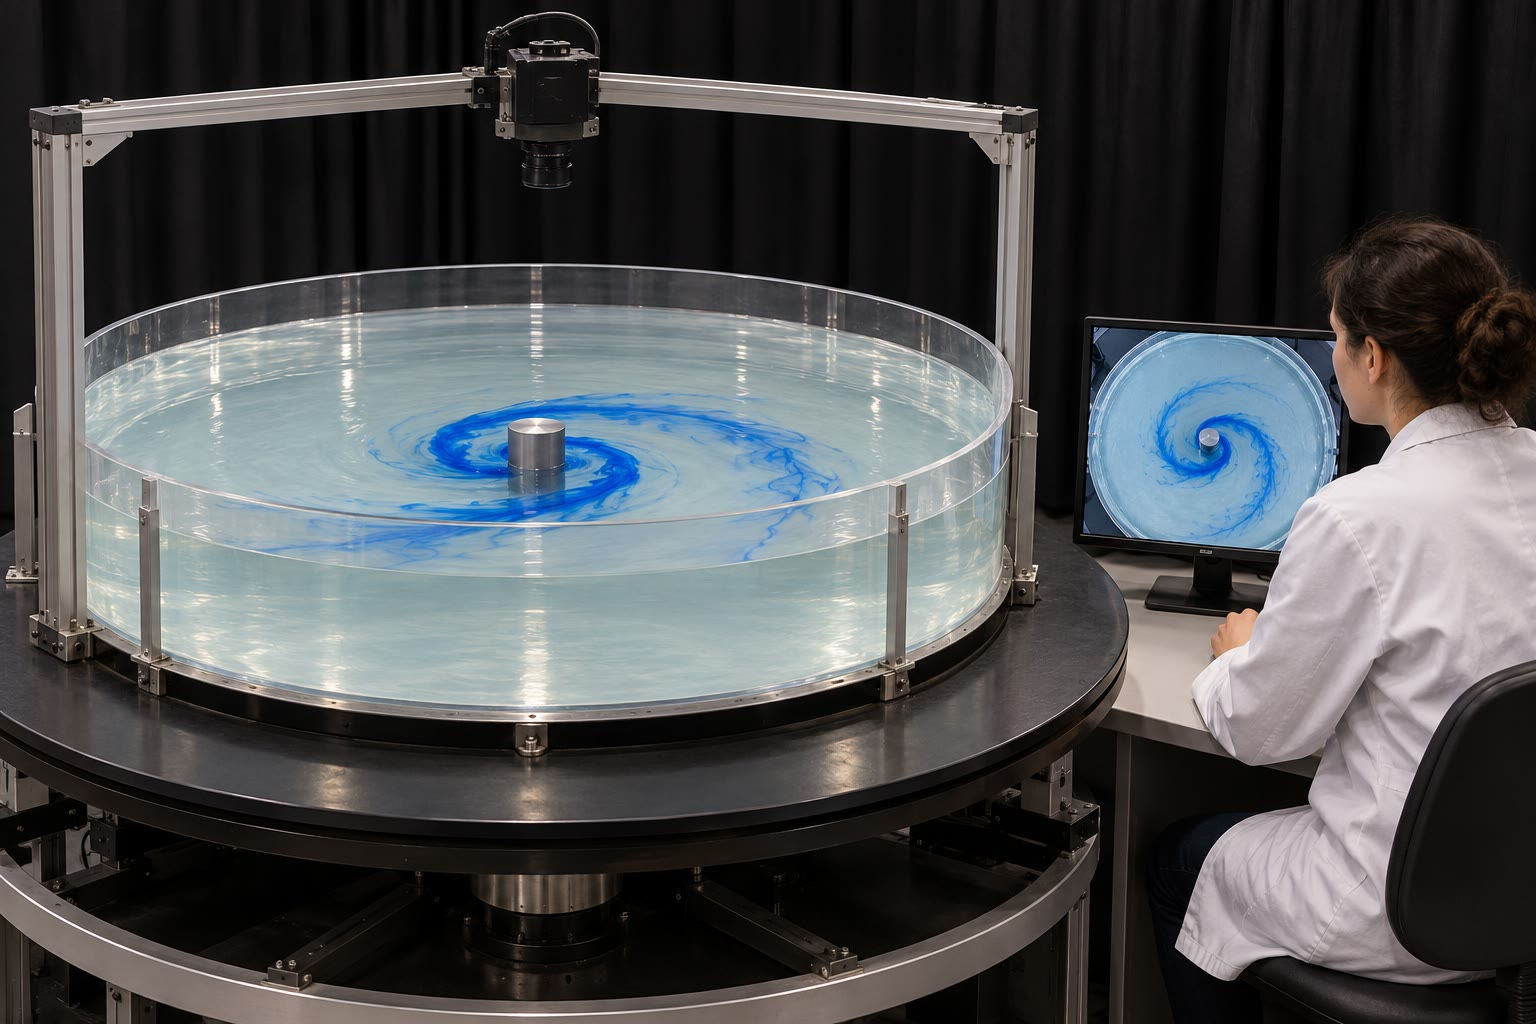
\includegraphics[width=\linewidth]{images/book5/ai/b3-rotating-tank.jpg}

{\scriptsize Um tanque girante: corante em espiral ao redor de um cilindro, filmado por uma
câmera que gira junto com a mesa (Ilustração gerada por IA.)}
\end{minipage}
\end{inthelab}

\section{Exercícios}

\begin{exercise}[$\star$]\label{exo:b3:gfd-foundations:1}
Tome $\Omega = \qty{7.292115e-5}{rad/s}$. (a)~Calcule o parâmetro de Coriolis
e o período inercial a \ang{30}, \ang{45} e \ang{60} N.
(b)~Calcule o raio do círculo inercial de uma corrente de
\qty{0.20}{m/s} nas mesmas latitudes. (c)~Compare o período inercial a
\ang{30} com o dia sideral, \qty{23.9345}{h}.
\end{exercise}

\begin{exercise}[$\star$]\label{exo:b3:gfd-foundations:2}
A \ang{45} N, calcule o \omterm{def:b3:gfd-foundations:numbers}{número de Rossby} de um redemoinho de poeira (\qty{10}{m/s},
\qty{10}{m}), de uma brisa marítima (\qty{5}{m/s}, \qty{20}{km}), de uma depressão
(\qty{15}{m/s}, \qty{1000}{km}) e de um giro oceânico (\qty{0.05}{m/s},
\qty{2000}{km}). Quais deles estão próximos do equilíbrio geostrófico?
\end{exercise}

\begin{exercise}[$\star$]\label{exo:b3:gfd-foundations:3}
A \ang{45} N, a temperatura média da troposfera, \qty{250}{K}, diminui
em direção ao norte \qty{5}{K} a cada \qty{1000}{km}. Usando o primeiro termo do
\omterm{thm:b3:gfd-foundations:thermal-wind}{vento térmico} em altura, calcule o cisalhamento vertical do vento de oeste e
o aumento do vento ao longo de \qty{10}{km}.
\end{exercise}

\begin{exercise}[$\star$]\label{exo:b3:gfd-foundations:4}
A estabilidade $E = -(1/\rho)\,\mathrm d\rho_\theta/\mathrm dz$ do quilômetro superior do
oceano situa-se entre \num{50e-8} e \qty{1000e-8}{m^{-1}};
em fossas oceânicas profundas, vale \qty{e-8}{m^{-1}}. Calcule $N = \sqrt{gE}$, o
período da oscilação de flutuabilidade e $N$ em ciclos por hora para estes
três valores.
\end{exercise}

\begin{exercise}[$\star\star$]\label{exo:b3:gfd-foundations:5}
Um sistema meteorológico tem $U = \qty{10}{m/s}$, $L = \qty{1000}{km}$, $H =
\qty{10}{km}$, a \ang{45} N. (a)~Estime sua velocidade vertical e sua
aceleração vertical, e compare esta última com $g$ e com o
gradiente vertical da perturbação de pressão, $fUL/H$. (b)~Calcule o
termo de Coriolis descartado $\tilde fu$ e compare-o com $g$.
\end{exercise}

\begin{exercise}[$\star\star$]\label{exo:b3:gfd-foundations:6}
Tome $f = \qty{e-4}{s^{-1}}$ e isóbaras circulares de raio
\qty{300}{km}. (a)~O gradiente de pressão ao redor de uma baixa dá $V_g =
\qty{20}{m/s}$: calcule o \omterm{def:b3:gfd-foundations:gradient}{vento gradiente}. (b)~Ao redor de uma alta,
$V_g = \qty{5}{m/s}$: calcule o \omterm{def:b3:gfd-foundations:gradient}{vento gradiente}. (c)~Qual é o maior
$V_g$ possível ao redor da alta, e qual é então o vento?
\end{exercise}

\begin{exercise}[$\star\star$]\label{exo:b3:gfd-foundations:7}
Um tanque de \qty{20}{cm} de profundidade gira uma vez a cada \qty{6}{s}; sua água tem $\nu =
\qty{e-6}{m^2/s}$. (a)~Calcule $f = 2\Omega$, depois o \omterm{def:b3:gfd-foundations:numbers}{número de Rossby} de um
escoamento de \qty{1}{cm/s} passando por um cilindro de \qty{5}{cm} de diâmetro, e o \omterm{def:b3:gfd-foundations:numbers}{número de Ekman}
do tanque. Vai se formar uma \omterm{thm:b3:gfd-foundations:taylor-proudman}{coluna de Taylor}? (b)~A teoria dá um tempo de spin-up
$H/\sqrt{\nu\Omega}$: calcule-o em minutos e em voltas da mesa.
\end{exercise}

\begin{exercise}[$\star\star$]\label{exo:b3:gfd-foundations:8}
Na média zonal de janeiro de 1991--2020, o vento de oeste é \qty{4.27}{m/s}
a \qty{850}{hPa} e \qty{40.39}{m/s} a \qty{250}{hPa} a \ang{30} N,
\qty{5.99}{m/s} e \qty{23.17}{m/s} a \ang{45} N. Com $R =
\qty{286.9}{J.kg^{-1}.K^{-1}}$, calcule o gradiente meridional da
temperatura média da camada nas duas latitudes, e diga por que o jato é mais intenso
a \ang{30} N.
\end{exercise}

\begin{exercise}[$\star\star$]\label{exo:b3:gfd-foundations:9}
(a)~Calcule o \omterm{def:b3:gfd-foundations:rossby-radius}{raio de deformação de Rossby} da troposfera ($N =
\qty{0.0113}{s^{-1}}$, $H = \qty{11}{km}$, \ang{45} N) e o da camada superior
do oceano ($N = \qty{0.00357}{s^{-1}}$, $H = \qty{1000}{m}$, \ang{40.5} N).
(b)~Com $a = \qty{6371}{km}$, calcule $\beta$ nas duas latitudes e a
variação relativa $\beta L_R/f$ do parâmetro de Coriolis sobre cada raio.
\end{exercise}

\begin{exercise}[$\star\star\star$]\label{exo:b3:gfd-foundations:10}
Uma parcela da superfície do oceano, posta em movimento com velocidade $U$, é freada
por atrito linear: $\mathrm du/\mathrm dt = fv - ru$, $\mathrm dv/\mathrm dt = -fu -
rv$. (a)~Resolva com $w = u + \mathrm iv$ e descreva a trajetória. (b)~A
parcela também é arrastada por uma corrente estacionária $u_0$ para leste: dê sua
posição. (c)~A \ang{45} N, com $U = \qty{0.2}{m/s}$, $r^{-1} =
\num{4}\text{ dias}$ e $u_0 = \qty{0.05}{m/s}$, dê sua velocidade em relação à
corrente após quatro dias e a distância que ela derivou.
\end{exercise}

\begin{exercise}[$\star\star\star$]\label{exo:b3:gfd-foundations:11}
Através de uma frente oceânica a \ang{40} N, a densidade da água aumenta
em direção ao norte \qty{1}{kg/m^3} ao longo de \qty{100}{km}, na camada superior
de \qty{1000}{m}; abaixo, a água é uniforme e parada. Com $\rho_0 =
\qty{1025}{kg/m^3}$, calcule o cisalhamento vertical da corrente e a
corrente na superfície. Em que direção ela flui?
\end{exercise}

\begin{exercise}[$\star\star\star$]\label{exo:b3:gfd-foundations:12}
A coluna de média anual a \ang{40.5} N, \ang{30.5} O apresenta densidades potenciais
$\sigma_\theta = \rho_\theta - \qty{1000}{kg/m^3}$ de 26.029 na
superfície, 26.697 a \qty{100}{m}, 27.079 a \qty{500}{m} e 27.628 a
\qty{1000}{m}. (a)~Calcule $N$ em cada uma das três camadas, em
\unit{s^{-1}} e em ciclos por hora. (b)~Qual camada é a mais estável,
e por quê? (c)~Compare os valores com a faixa do oceano superior indicada
no \cref{exo:b3:gfd-foundations:4}.
\end{exercise}
% ledger: geod5:grs80-defining, earth:Trot, stewart:stability, data:b5-ncep-uwnd, data:b5-woa23-atlantic, earth:Rmean

\section{Problema: ventos sobre a estepe de Orrin}

\begin{problem}[{Problema de fim de semana --- a rotação, a estratificação e
os ventos de uma planície inventada a \ang{48} N}]
\label{pb:b3:gfd-foundations:1}
A estepe de Orrin é uma planície plana a \ang{48} N, com um lago, o lago Orrin,
com \qty{12}{km} de largura, e um pequeno laboratório com um tanque giratório. Tome
$\Omega = \qty{7.292115e-5}{rad/s}$, $g = \qty{9.81}{m/s^2}$, $R =
\qty{286.9}{J.kg^{-1}.K^{-1}}$ e $c_p = \qty{1004}{J.kg^{-1}.K^{-1}}$.
Todos os valores da estepe, de seu lago e de seus ventos são inventados.

\medskip\noindent\textbf{Parte I --- A rotação importa?}
\begin{enumerate}
\item Calcule o parâmetro de Coriolis e o período inercial em Orrin.
\item Calcule o \omterm{def:b3:gfd-foundations:numbers}{número de Rossby} de cinco escoamentos: água escoando de uma banheira
  (\qty{0.1}{m/s} sobre \qty{0.3}{m}); o tanque do laboratório, que dá uma volta
  a cada \qty{10}{s} (com $f = 2\Omega_{\text{tanque}}$; \qty{5}{mm/s}
  sobre \qty{0.2}{m}); a brisa da tarde vinda do lago (\qty{5}{m/s},
  \qty{20}{km}); uma depressão (\qty{15}{m/s}, \qty{1000}{km}); o giro de uma
  bacia oceânica na mesma latitude (\qty{0.05}{m/s}, \qty{2000}{km}).
\item Quais desses escoamentos sentem a rotação que os impulsiona, e quais estão
  próximos do geostrófico?
\item Calcule o \omterm{def:b3:gfd-foundations:numbers}{número de Ekman} do tanque (\qty{0.2}{m} de profundidade, $\nu =
  \qty{e-6}{m^2/s}$), da depressão (viscosidade turbulenta de \qty{10}{m^2/s},
  profundidade de \qty{10}{km}) e do giro (viscosidade turbulenta de \qty{e-3}{m^2/s},
  profundidade de \qty{1000}{m}).
\item A camada de Ekman tem espessura $\delta = \sqrt{2\nu/f}$. Mostre que
  $\delta/H = \sqrt{2\,\mathrm{Ek}}$ e calcule $\delta$ para o tanque e para
  o ar da estepe.
\item O que esses números dizem sobre onde o atrito importa?
\end{enumerate}

\medskip\noindent\textbf{Parte II --- O vento junto ao solo.}
\begin{enumerate}[resume]
\item Junto ao solo a pressão é \qty{1012.9}{hPa} e a temperatura
  \qty{288.1}{K}. Calcule a densidade do ar.
\item A pressão ao nível do mar cai para o norte \qty{4}{hPa} a cada
  \qty{300}{km}. Calcule o vento geostrófico e indique sua direção.
\item O mesmo gradiente envolve uma depressão cujas isóbaras têm raio
  de \qty{600}{km}. Calcule o \omterm{def:b3:gfd-foundations:numbers}{número de Rossby} das isóbaras e o
  \omterm{def:b3:gfd-foundations:gradient}{vento gradiente}.
\item O mesmo gradiente envolve um anticiclone de mesmo raio.
  Calcule o \omterm{def:b3:gfd-foundations:gradient}{vento gradiente} e o maior gradiente de pressão, em
  \unit{hPa} a cada \qty{300}{km}, que o anticiclone pode sustentar.
\end{enumerate}

\medskip\noindent\textbf{Parte III --- Estratificação.}
\begin{enumerate}[resume]
\item A temperatura da troposfera cai \qty{6.49}{K/km}.
  Calcule o gradiente adiabático seco $g/c_p$, e $N$ e o período da
  oscilação de flutuabilidade a \qty{5}{km}, onde a temperatura é
  \qty{255.7}{K}.
\item Acima de \qty{11}{km} o ar é isotérmico a \qty{216.6}{K}. Mostre que
  $N^2 = g^2/(c_pT)$ ali, e calcule $N$ e sua razão para o valor da
  questão~11.
\item Calcule o \omterm{def:b3:gfd-foundations:rossby-radius}{raio de deformação de Rossby} da troposfera de Orrin, com o $N$ da
  questão~11 e $H = \qty{10}{km}$, e compare-o com o tamanho da
  depressão da Parte~I.
\item No verão, os \qty{20}{m} superiores do lago Orrin são mais leves que a
  água profunda em \qty{1.5}{kg/m^3} ($\rho_0 = \qty{1000}{kg/m^3}$). Calcule
  a gravidade reduzida $g' = g\,\Delta\rho/\rho_0$, a velocidade $\sqrt{g'h}$ das
  ondas internas lentas da camada superior e o \omterm{def:b3:gfd-foundations:rossby-radius}{raio de deformação de Rossby}
  $\sqrt{g'h}/f$.
\item A rotação da Terra vai moldar os movimentos internos do lago?
\end{enumerate}

\medskip\noindent\textbf{Parte IV --- O vento térmico.}
\begin{enumerate}[resume]
\item Duas estações de radiossondagem distam \qty{600}{km} entre si, sobre o mesmo
  meridiano. A temperatura média da camada desde o solo,
  \qty{1013}{hPa}, até \qty{265}{hPa}, cerca de \qty{10}{km}, é \qty{253.0}{K}
  na estação do sul e \qty{249.4}{K} na do norte. Calcule o
  gradiente meridional de temperatura em \unit{K} por \qty{1000}{km}.
\item A espessura de uma camada entre duas pressões é $\Delta z = (R\bar
  T/g)\ln(p_b/p_t)$. Calcule-a nas duas estações, e a inclinação da
  superfície de \qty{265}{hPa} em relação à superfície ao nível do solo.
\item Deduza o aumento do vento geostrófico do solo até
  \qty{265}{hPa}, a partir dessa inclinação.
\item Calcule o mesmo aumento com o teorema do \omterm{thm:b3:gfd-foundations:thermal-wind}{vento térmico} em pressão.
\item O ar da estepe é \omterm{def:b3:gfd-foundations:baroclinic}{barotrópico} ou \omterm{def:b3:gfd-foundations:baroclinic}{baroclínico}? Qual seria o vento
  a \qty{265}{hPa} se fosse \omterm{def:b3:gfd-foundations:baroclinic}{barotrópico}?
\item Calcule o aumento a partir do primeiro termo do \omterm{thm:b3:gfd-foundations:thermal-wind}{vento térmico} em
  altura, com a temperatura média da troposfera padrão entre 0
  e \qty{10}{km}, \qty{255.7}{K}, e compare.
\item Calcule o vento a \qty{541}{hPa}, cerca de \qty{5}{km}, supondo que o
  gradiente de temperatura seja o mesmo em todos os níveis.
\item O número de Richardson $N^2/(\partial u/\partial z)^2$ deve cair abaixo de
  0.25 para que o cisalhamento gere turbulência. Calcule-o para a troposfera de
  Orrin.
\item Em janeiro, a média zonal dos ventos de oeste a \qty{250}{hPa} é \qty{23.2}{m/s}
  a \ang{45} N e \qty{40.4}{m/s} a \ang{30} N. Compare com o vento de
  Orrin, e explique por que um vento local pode superar a média zonal.
\item Dê o vento geostrófico a \qty{10}{km} acima da estepe de Orrin.
\end{enumerate}
\end{problem}
% ledger: geod5:grs80-defining, stewart:stability, data:b5-ncep-uwnd, nasa:grc-atmos
